% CVPR 2023 Paper Template
% based on the CVPR template provided by Ming-Ming Cheng (https://github.com/MCG-NKU/CVPR_Template)
% modified and extended by Stefan Roth (stefan.roth@NOSPAMtu-darmstadt.de)

\documentclass[10pt,twocolumn,letterpaper]{article}

%%%%%%%%% PAPER TYPE  - PLEASE UPDATE FOR FINAL VERSION
% \usepackage[review]{cvpr}      % To produce the REVIEW version
\usepackage{cvpr}              % To produce the CAMERA-READY version
\usepackage{csc}
%\usepackage[pagenumbers]{cvpr} % To force page numbers, e.g. for an arXiv version

% Include other packages here, before hyperref.
\usepackage{graphicx}
\usepackage{amsmath}
\usepackage{amssymb}
\usepackage{booktabs}


% It is strongly recommended to use hyperref, especially for the review version.
% hyperref with option pagebackref eases the reviewers' job.
% Please disable hyperref *only* if you encounter grave issues, e.g. with the
% file validation for the camera-ready version.
%
% If you comment hyperref and then uncomment it, you should delete
% ReviewTempalte.aux before re-running LaTeX.
% (Or just hit 'q' on the first LaTeX run, let it finish, and you
%  should be clear).
\usepackage[pagebackref,breaklinks,colorlinks]{hyperref}


% Support for easy cross-referencing
\usepackage[capitalize]{cleveref}
\crefname{section}{Sec.}{Secs.}
\Crefname{section}{Section}{Sections}
\Crefname{table}{Table}{Tables}
\crefname{table}{Tab.}{Tabs.}


%%%%%%%%% PAPER ID  - PLEASE UPDATE
\def\cvprPaperID{*****} % *** Enter the CVPR Paper ID here
\def\confName{CVPR}
\def\confYear{2023}


\begin{document}

%%%%%%%%% TITLE - PLEASE UPDATE
\title{CSC2530 Project Report}

\author{Jason Tang (tangja10)\\
University of Toronto\\
{\tt\small jasontang@cs.toronto.edu}
}
\maketitle

%%%%%%%%% ABSTRACT
\begin{abstract}
  In this paper, we explore the use of a stereoscopic depth sensor to estimate an initial point cloud for the Point-NeRF method, an extension of Neural Radiance Fields (NeRF) that optimizes the training and inference processes by sampling points near an estimated point cloud. We develop experimental modifications and conduct real-world experiments to analyze the impact of incorporating a coarsely estimated point cloud on the performance and efficiency of Point-NeRF. Our results suggest that incorporating stereoscopic depth sensors into the Point-NeRF 3D scene reconstruction pipeline has the potential to enhance the quality of novel view synthesized images, while still maintaining the sample efficiency improvements provided by Point-NeRF.
\end{abstract}

%%%%%%%%% BODY TEXT
\section{Introduction}
\label{sec:intro}
Neural Radiance Fields (NeRF) \cite{NeRF} have gained significant attention recently for their impressive ability to generate high-fidelity novel views and realistic 3D renderings of scenes using only a collection of 2D images captured from multiple viewpoints. In particular, NeRF employs a multi-layer perceptron (MLP) network to predict color and density, based on the location and viewing direction, which is then used to reconstruct the entire scene.

To address the large number of empty points within the scene, NeRF first performs a coarse analysis to detect relevant parts of the scene, followed by a finer analysis on the selected portions. Despite this, a significant amount of computational time is still wasted on processing irrelevant, low-density points. As such, the computational requirements for training NeRFs pose a significant challenge for a wide range of practical applications and is an active area of research \cite{EfficientNeRF}.

Faster NeRF training and inference times can have significant implications for a variety of applications, including film production, augmented reality, and autonomous systems. Improved sample efficiency can enable faster generation of realistic 3D scenes, enhanced immersive experiences for users, and precise environmental perception in autonomous vehicles. 

Numerous extensions have been made to further optimize the training and inference processes of NeRF, usually by running the MLP at fewer, but higher quality points. In this project, we will analyze one such extension called Point-NeRF \cite{PointNeRF}, which only samples points near an estimated point cloud. Specifically, we will assess the empirical performance of using a stereoscopic depth sensor (Intel RealSense Depth Camera D435) to estimate an initial point cloud compared to other point cloud estimation methods.



\section{Related Work}
\label{sec:related}

\subsection{NeRF}
Mildenhall et al. presented the foundational NeRF method in 2020 \cite{NeRF}, which proposed a new method for synthesizing novel views of a scene from a small number of input images by representing scenes as Neural Radiance Fields. This proposed method involves training a multilayer perceptron (MLP) network to learn a continuous 5D function that maps 3D spatial coordinates $(x, y, z)$ and 2D viewing directions $(\theta, \phi)$ to a volume density and RGB color. 

To train the NeRF model, the authors sample 3D points along rays emanating from the input viewing angle and position for each pixel, generate output densities and colors, and integrate samples along each ray into a single pixel color using differentiable volume rendering techniques. They then minimize the L2 norm between the rendered images and the ground truth images from the training set. 

\newcommand{\cc}{\textbf{c}}
\newcommand{\rr}{\textbf{r}}
\newcommand{\oo}{\textbf{o}}
\newcommand{\dd}{\textbf{d}}
\newcommand{\xx}{\textbf{x}}
In particular, the volume density $\sigma(\xx)$ only depends on spatial location $\xx = (x, y, z)$, whereas the output color $\cc(\xx, \dd)$ depends on both spatial location $\xx$ and viewing direction $\dd = (\theta, \phi)$. The pixel color of each ray $\rr(t) = \oo + t\dd$ is then given by the integral of the product of the volume density and color along the ray:
\begin{align*}
  &C(\rr) = \int_{t_n}^{t_f} T(t) \sigma(\rr(t)) \cc(\rr(t), \dd) dt 
  \tag{1}\\
  &\text{where } T(t) = \exp\left(-\int_{t_n}^{t} \sigma(\rr(s)) ds\right)
\end{align*}
where $t_n$ and $t_f$ are the near and far bounds, respectively. 

% This function calculates the color of a pixel by assigning weights to the color of each sampled point proportional to its density and inversely proportional to the density of sampled points preceding it along the ray. 
The authors use quadrature to numerically estimate this integral, with samples drawn uniformly from evenly spaced bins along the ray. This enables the MLP to learn a continuous representation as the samples are situated on a continuous domain throughout training.

To improve sampling efficiency, the authors begin by generating a coarse, evenly spaced set of points along each ray, which is then used to direct a finer sampling of points towards the more relevant and higher density segments of the ray. They also employ positional encoding of the 5D input to further enhance the resolution at which the MLP can learn to represent.

The empirical results demonstrated that NeRF was effective in generating new views, both in synthetic datasets such as DeepVoxels and a newly developed dataset in this paper, as well as complex real-world scenes such as LLFF and several manually captured scenes. Compared to prior state-of-the-art methods, NeRF showed significant improvement and did not require ground truth 3D geometry, enabling its use in higher complexity real-world datasets. Moreover, NeRF was able to achieve higher resolutions due to its improved sampling efficiency, which was not previously possible due to time and space constraints imposed by finer sampling requirements. 

However, even with its improved efficiency, training NeRF still requires a significant amount of time, with convergence taking between 1 to 2 days on an NVIDIA V100 GPU. 



\subsection{Point-NeRF}
Point-NeRF \cite{PointNeRF} is a method that leverages an estimated point cloud to enhance sample efficiency by selectively sampling points that are near the prior cloud and have a higher likelihood of being relevant. To generate the initial point cloud from the collection of input images, the authors utilize existing multi-view reconstruction methods, such as COLMAP \cite{COLMAP} or the deep learning based Multi-View Stereo Networks (MVSNet) \cite{MVSNet}. Afterward, learnable neural features are mapped to each point by a neural points model, which can utilize pretrained weights to accelerate training time and utilize auxiliary knowledge. 

During inference for a given sample point, Point-NeRF combines the viewing angle with an aggregation of the neural features of the $k$ nearest neighboring points, along with their confidence scores of being non-noisy and their relative positions with respect to the inference point. As a result, Point-NeRF achieves improved sampling efficiency, and is able to store local spatial information within neural points, thereby reducing the burden on the global model to memorize all the details within the scene. 

Additionally, Point-NeRF also has the capability to remove points with low confidence (likely noisy) and add points to fill in holes which are commonly found in point clouds estimated using stereopsis. This results in improved scalability, fast convergence, and higher rendering quality compared to the standard NeRF method.


%%%%%%% 
\begin{figure}[b]
  \centering
  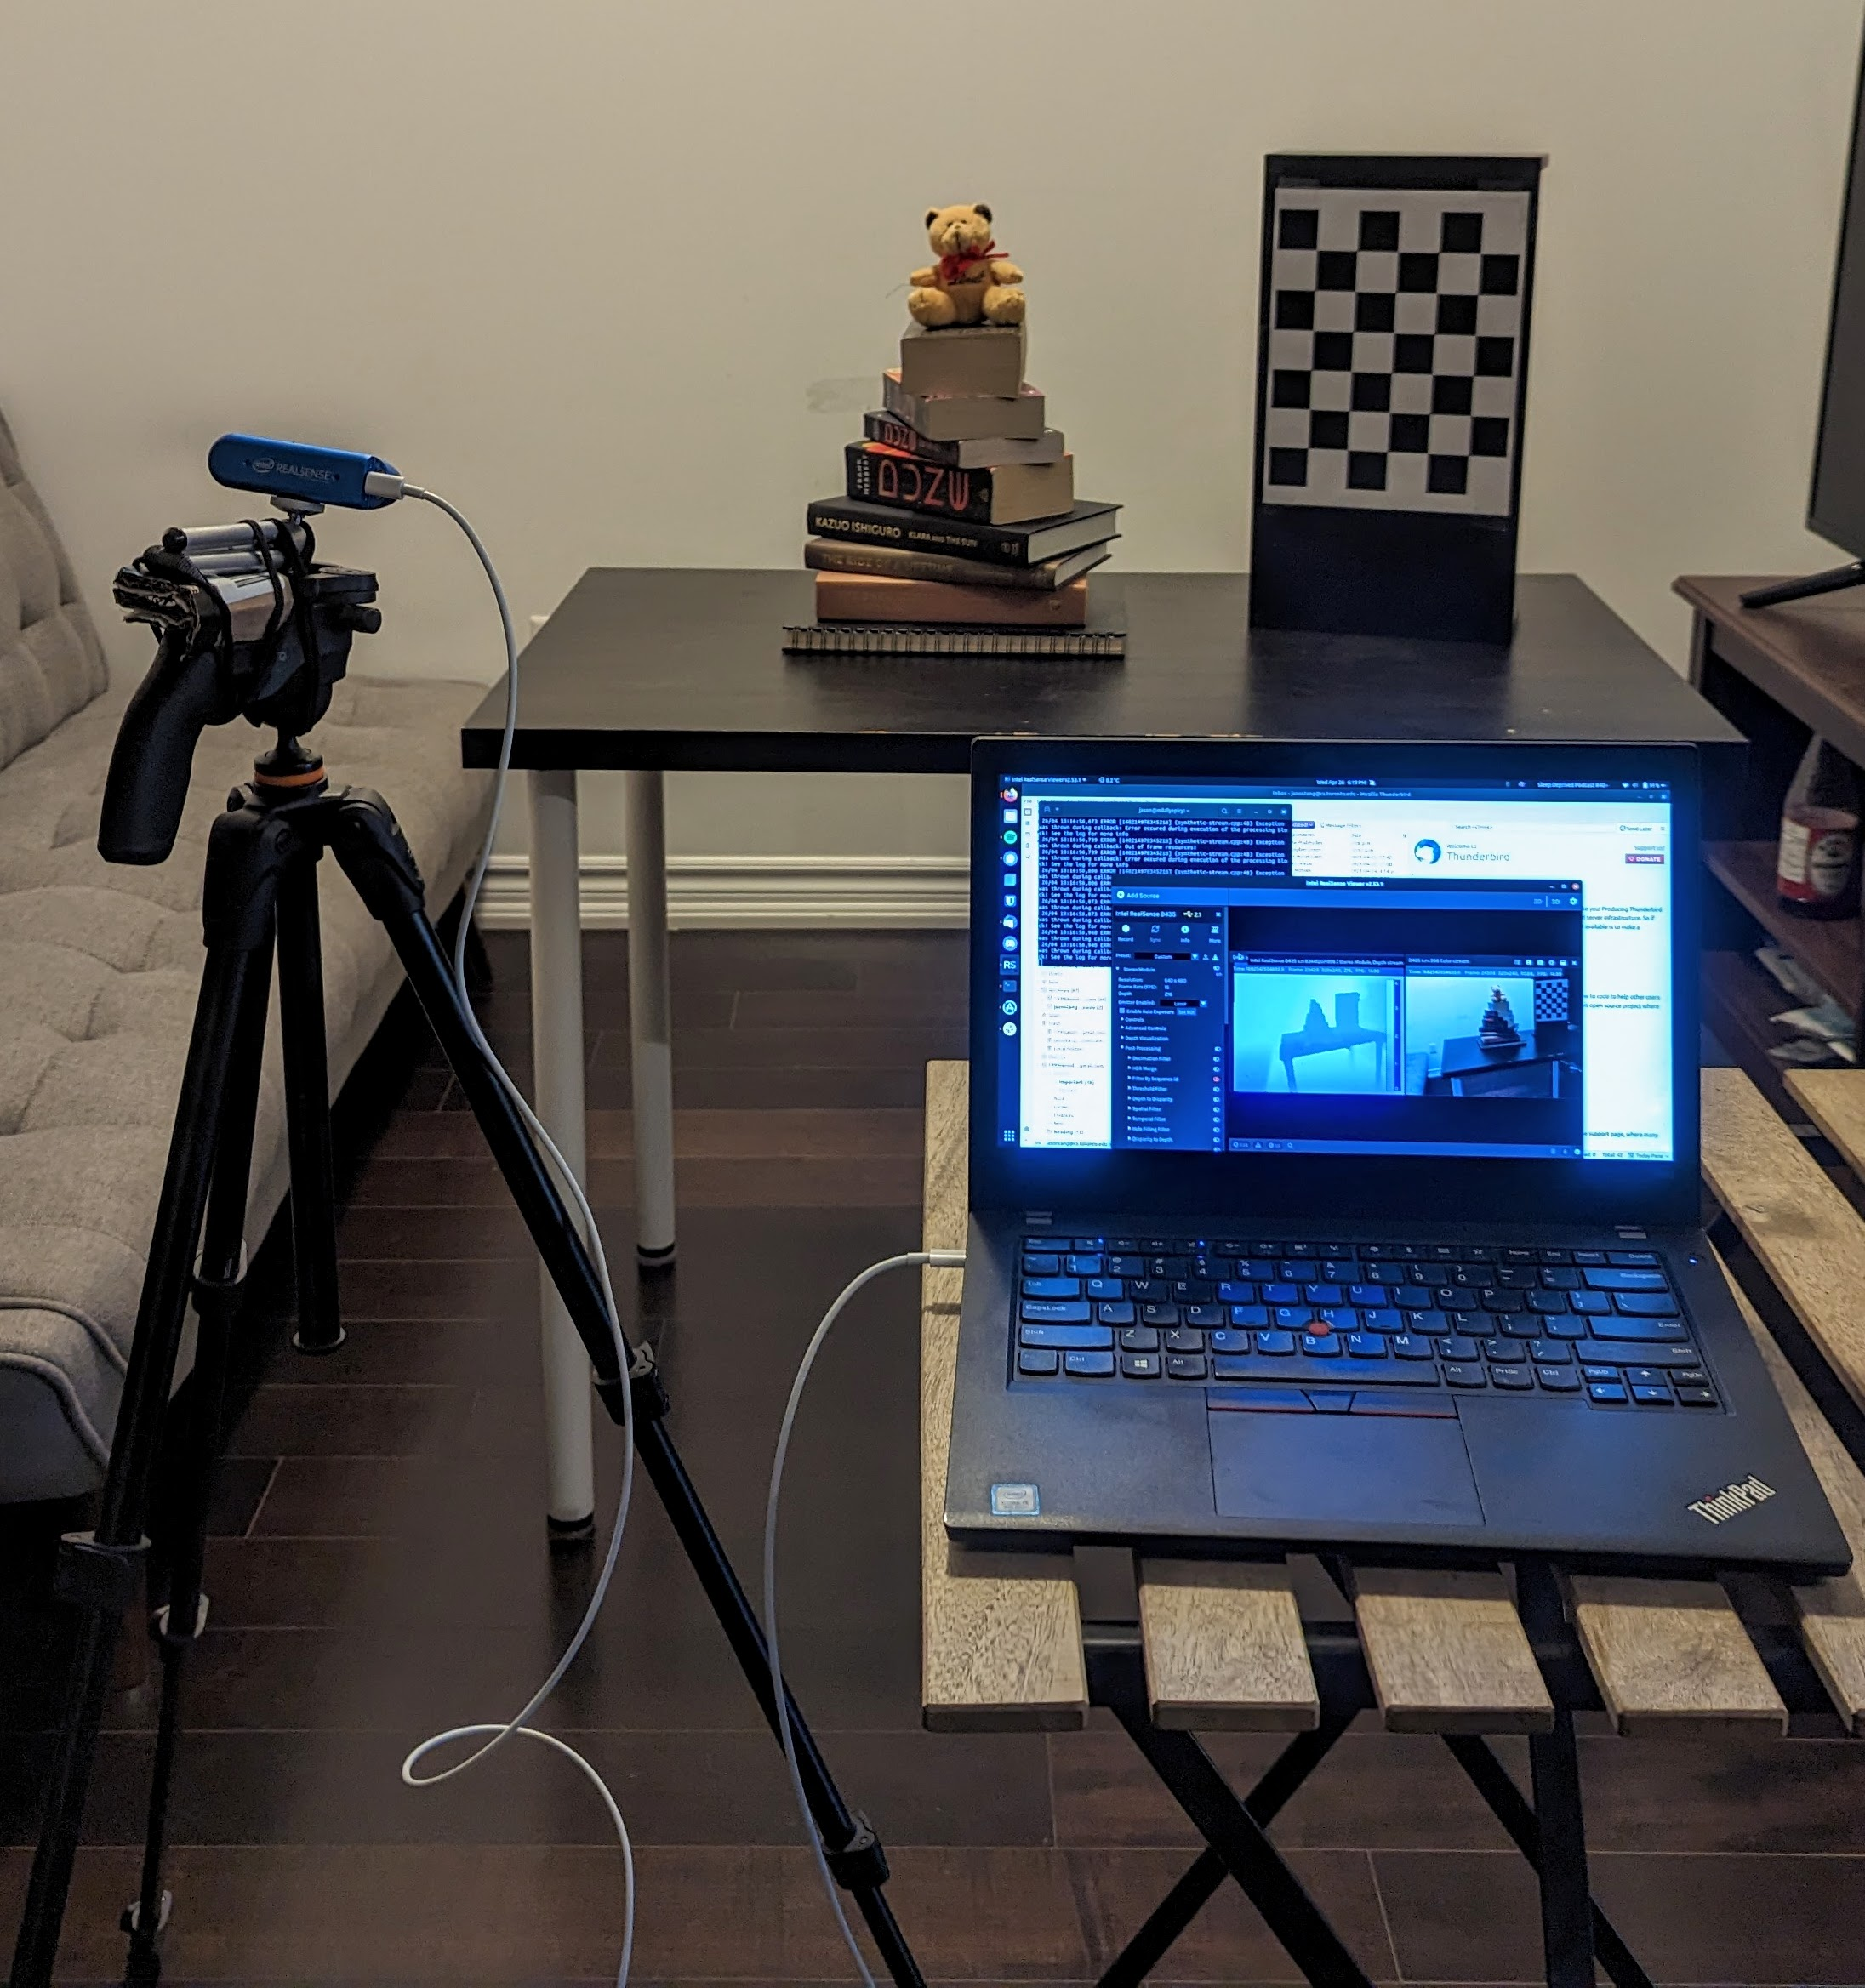
\includegraphics[width=0.8\linewidth]{images/setup.jpg}
  \caption{Scene capturing setup for the "books" scene.}
   \label{fig:setup}
\end{figure}

\subsection{Multi-View Reconstruction}
Extensive research has been conducted in the area of converting multi-view image collections into 3D point clouds, with notable contributions including methods such as COLMAP \cite{COLMAP} and Multi-View Stereo Network (MVSNet) \cite{MVSNet}.

COLMAP \cite{COLMAP} is a photogrammetric 3D reconstruction method, which estimates the 3D position of points in a scene using triangulation from multiple input images. To achieve this, COLMAP first detects and matches features in the input images, then performs a sparse reconstruction by estimating the 3D position of these features, and finally refines the reconstruction by performing bundle adjustment to minimize the reprojection error between the estimated 3D points and their corresponding 2D image points. Following this, COLMAP is able to perform a dense point cloud reconstruction by estimating the 3D positions for all pixels in each image, using the computed sparse reconstruction and the camera calibration parameters.

MVSNet \cite{MVSNet} is a popular deep learning approach to scene depth reconstruction. It begins by utilizing a convolutional neural network (CNN) to extract deep features from images, which are then warped through differentiable homographies and generates 3D feature volumes containing matching costs between two images. These feature volumes are then aggregated into a single cost volume using a variance-based cost metric to measure multi-view feature differences. This cost volume is then regularized utilizing a multi-scale 3D CNN similar to UNet \cite{UNet}, and a confidence map of depth hypotheses is generated. Lastly, the output depth maps are estimated using a differentiable soft argmin operation. The fully differentiable architecture of MVSNet enables end-to-end learning, leading to outstanding performance on standard benchmark datasets.

Despite their successes and popularity, these approaches still produce noisy outlier points or holes in the final point cloud, which are challenging to rectify through post-processing.




\subsection{Similar NeRF Extensions}
\subsubsection{EfficientNeRF}
EfficientNeRF \cite{EfficientNeRF} is another NeRF extension which also aims to improve sampling efficiency through two new strategies, Valid Sampling for the coarse stage and Pivotal Sampling for the fine stage. Overall, EfficientNeRF is able to speed up the training process by up to 10 times.

In vanilla NeRF, only a small proportion ($\sim 10-20\%$) of the uniformly sampled coarse points contribute to the final rendering result. As such, EfficientNeRF only uses “valid samples”, which are defined as points with a non-zero density. To obtain these densities, the authors store and query a set of momentum density voxels, which reflect the latest density distribution over the whole scene and are smoothed using momentum. As a result, EfficientNeRF can quickly obtain the density of a given 3D point through querying rather than a forward pass in the MLP. 

For the fine stage, the authors propose Pivotal Sampling, a method which only considers samples with a weight greater than a small threshold value. Each sample weight is inversely proportional to the previous coarse weights along the ray, and proportional to the density of the sample. Through this, the authors are able to finely sample points along each ray which are more likely to be relevant in the final rendering. 

\subsubsection{PixelNeRF}
PixelNeRF \cite{PixelNeRF} takes a different approach compared to Point-NeRF by first using a deep convolutional network to create spatial image features aligned to individual pixels, and then aggregating the traced pixel features from multiple views and feeding the result into the global MLP. This also allows for initialization with pretrained weights, but does not improve sampling efficiency over vanilla NeRF, meaning a significant amount of computation is still wasted on low density points.









\begin{figure}[t]
  \centering
  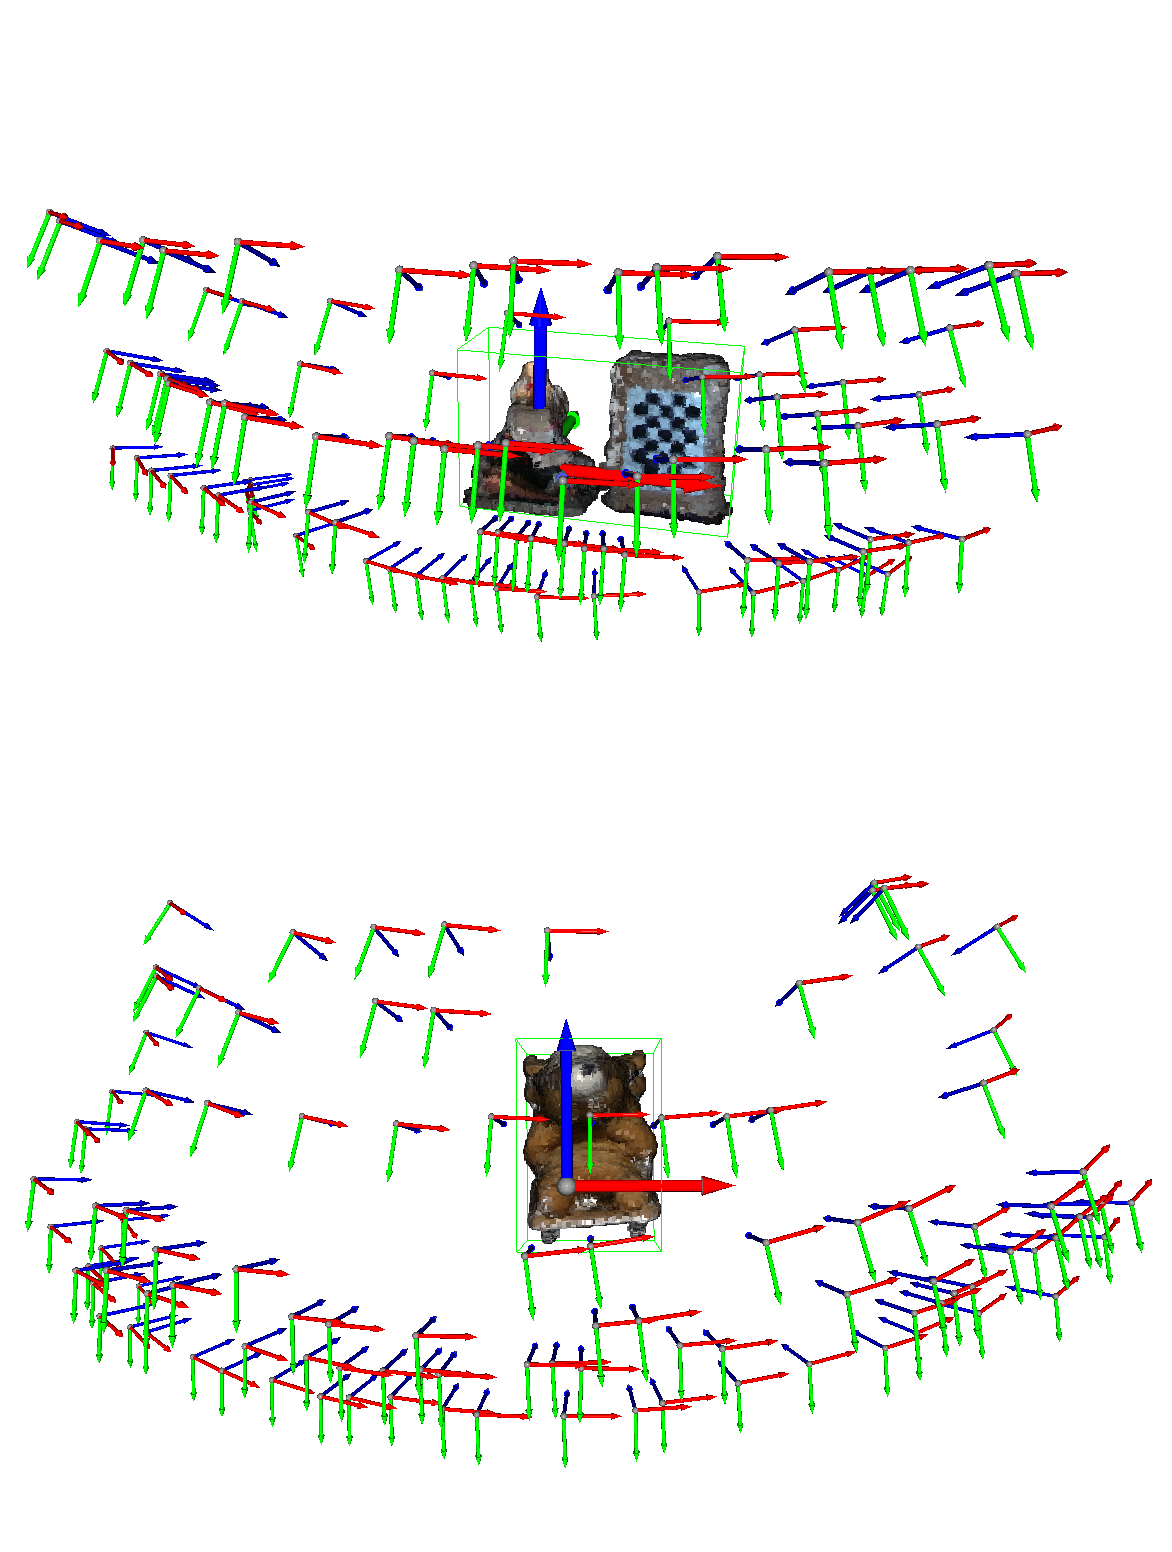
\includegraphics[width=0.8\linewidth]{images/cams.png}
  \caption{Camera poses for "books" (top) and "bear" (bottom) scenes.}
   \label{fig:cams}
\end{figure}




\begin{figure*}[ht!]
  \centering
  \begin{subfigure}{\linewidth}
    \centering
    \includegraphics[width=0.8\linewidth]{images/books.png}
    \caption{Novel View Rendering on Books Scene (250,000 iterations).}
  \end{subfigure}
  
  \begin{subfigure}{\linewidth}
    \centering
    \includegraphics[width=0.8\linewidth]{images/bear.png}
    \caption{Novel View Rendering on Bear Scene (200,000 iterations).}
  \end{subfigure}
  \caption{Ground Truth Test Images with Point-NeRF renderings under 2 different initializations.}
  \label{fig:test}
\end{figure*}
% %%%%%%%%%%%%%%%%%%%%%%%%%%
\section{Theory}
\label{sec:overview}
Stereoscopic depth sensors are small and cost-effective devices that can be easily integrated into 3D scene reconstruction setups on devices such as drones, cameras, and robots. Given these practical advantages, we investigate the performance of Point-NeRF in various real-world scenarios and analyze the effects of possible improvements, such as initializing or regularizing the model using an initial estimated point cloud obtained from a stereoscopic depth camera.

To train the Point-NeRF model using an acquired point cloud, we develop our experimental modifications on top of the \href{https://github.com/Xharlie/pointnerf}{official Point-NeRF Implementation}\footnote{https://github.com/Xharlie/pointnerf}. 
The Point-NeRF method requires processed RBGA images and calculated camera pose estimates as inputs to run. 

In our experiments, we use the alpha channel to mask irrelevant image backgrounds, thereby allowing the model to focus solely on representing the target and improving training efficiency. To find the relevant parts of the image, we try two methods: a classical approach of separating the two modes of near and far depths, and a more recent neural-based object segmentation approach called “U$^2$-Net” \cite{U2Net}. U$^2$-Net is based on a nested version of U-Net \cite{UNet}, and has been shown to be highly performant at object segmentation. We use an existing implementation in \href{https://github.com/danielgatis/rembg}{rembg}\footnote{https://github.com/danielgatis/rembg}.

For camera pose estimation, we experiment with both checkerboard alignment in openCV, as well as extracting camera pose estimates from \href{https://github.com/colmap/colmap}{COLMAP}\footnote{https://github.com/colmap/colmap}.
 
Overall, the objective of our project is to analyze the impact of incorporating a coarsely estimated point cloud on the performance and efficiency of Point-NeRF. To achieve this, we plan to obtain coarse depth maps with a stereoscopic depth sensor, generate 3D point clouds, and conduct real-world experiments to assess the performance of different configurations. 







\begin{figure*}[h!]
  \centering
  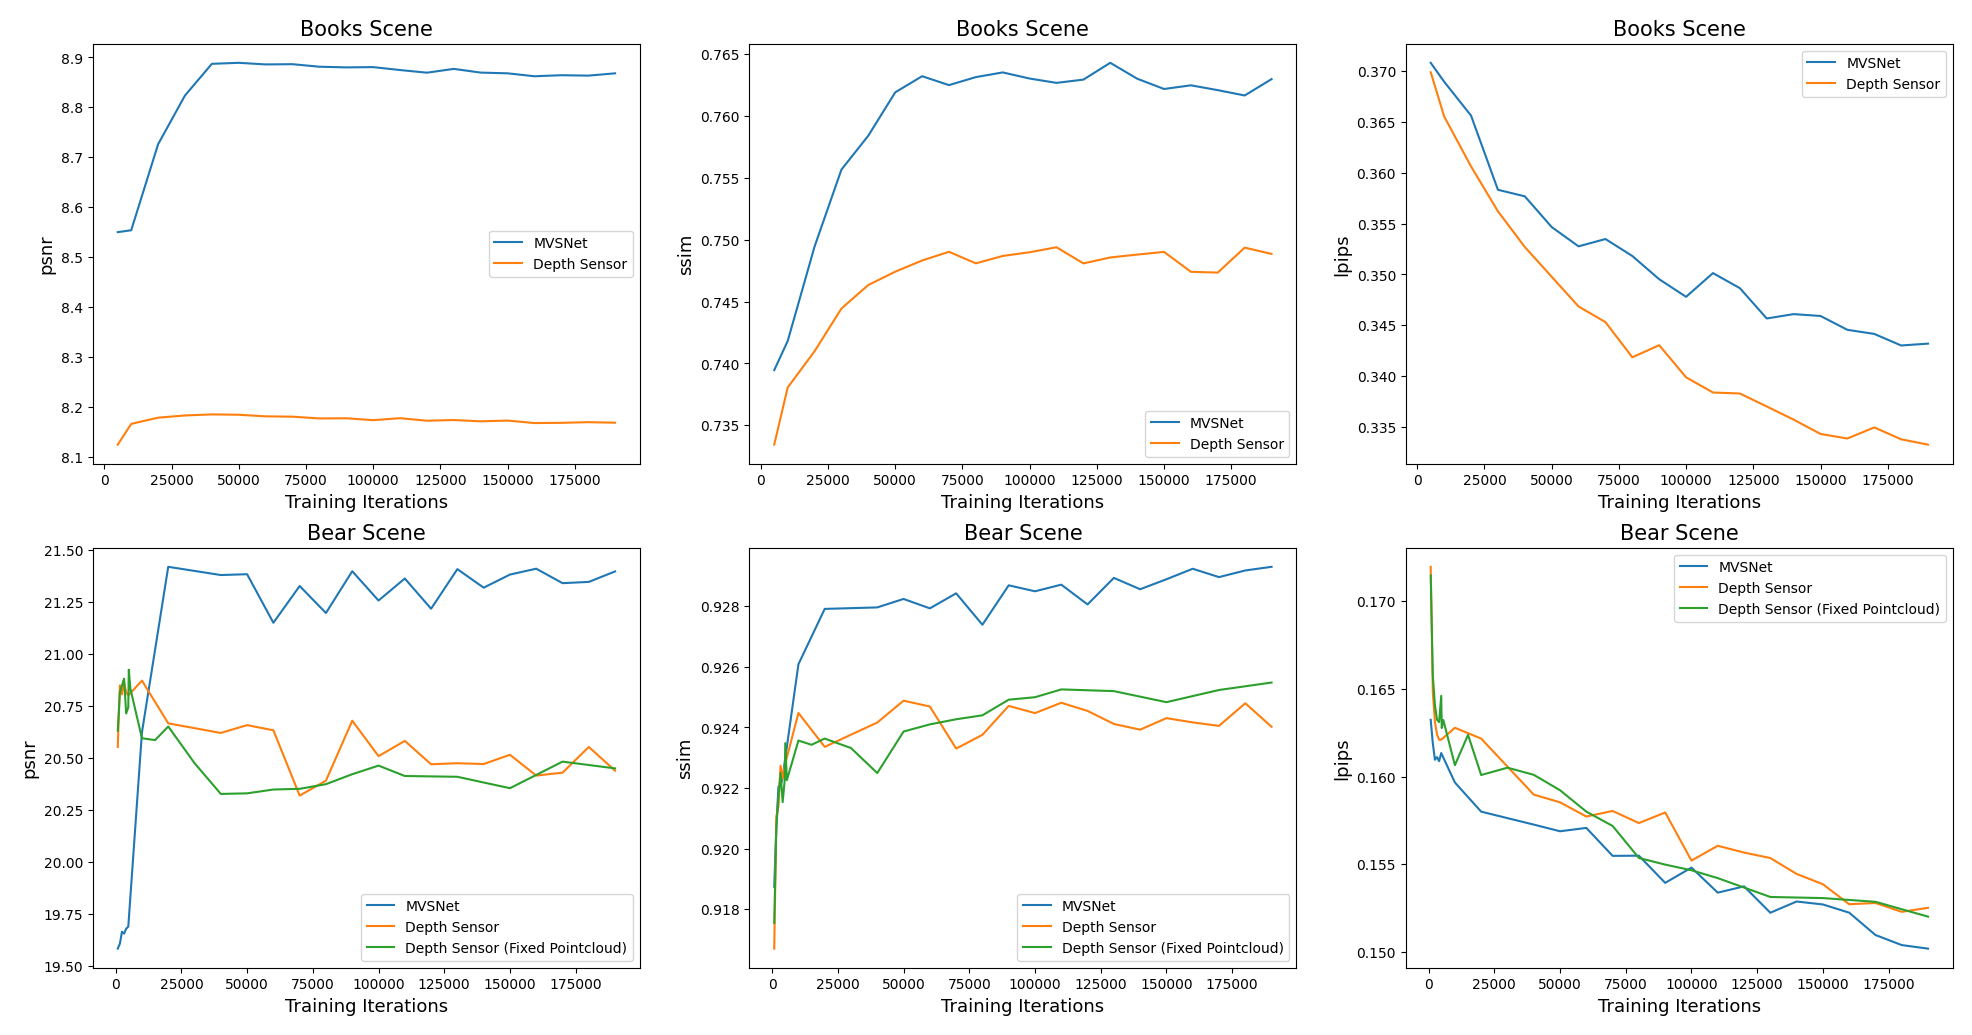
\includegraphics[width=\linewidth]{images/loss.png}
  \caption{Metrics during experiments.}
  \label{fig:loss}
\end{figure*}
%%%%%%%%%%%%%%%%%%%%%%%%%%%
\section{Analysis}
In our experiments, we utilized an Intel RealSense Stereoscopic Depth Camera (model D435) to capture both RGB and depth images which were then aligned and processed into an estimated point cloud. The D435 sensor works at an ideal range of 0.3 - 3m, which we stay within for all experiments, and we set it to output 640x480 RGB and 848x480 depth images. Besides the two cameras necessary for stereo vision, this sensor also contains an infrared ($\sim$850nm) laser projector system which is used to improve depth estimates of low texture surfaces such as walls. 
To reduce camera shake, we securely mounted the D435 sensor onto a camera tripod and used a wireless mouse to interact with the laptop when recording (see Fig \ref{fig:setup}).


We captured 2 scenes, “books” and “bear”, with 162 and 211 images taken from different angles facing the target object, respectively (see Fig \ref{fig:cams}). In “books”, we also placed a printed checkerboard pattern next to it for camera pose estimation (see Fig \ref{fig:setup}), whereas we relied only on COLMAP for pose estimation in “bear”. 

For metrics, we measure peak signal-to-noise ratio (PSNR) and Structural Similarity Index (SSIM), where a higher value is better, as well as Learned Perceptual Image Patch Similarity (LPIPS) \cite{LPIPS}, where a lower value is better (see Fig \ref{fig:loss}). PSNR is a commonly used metric to measure image quality as the ratio of the maximum signal power to the power of corrupting noise. Similarly, SSIM is commonly used to measure compression quality as structural similarities, such as luminance and contrast. LPIPS is a more recent metric which utilizes the similarity between activations of two images in a deep neural network, and has been shown to agree well with human perception. 

All code for our experiments are available at \href{https://github.com/JasonTang99/point-nerf-coarse-depth}{this GitHub repository}. All collected images are available on \href{https://drive.google.com/file/d/1GoUAKg_cYg8mOlF4c6UzspSZBblQxR9W/view?usp=sharing}{Google Drive}, and all experiment run checkpoints are also available on \href{https://drive.google.com/file/d/12V81zXsEQGoPJjw1pRJ4FXC-id6qfmXd/view?usp=sharing}{Google Drive}.



%%%%%%%%%%%%%%%%%%%%%%%%%%%
\section{Experimental Results}
During our experiments, we observed that processing our scenes with COLMAP took around 30-60 minutes, whereas using MVSNet took around 10-15 minutes to complete. Following this, we trained each Point-NeRF experiment for at least 200,000 iterations, as per the recommendations in the research paper. We ran our experiments on an NVIDIA RTX 3060 Ti with 8GB VRAM whereas most researchers run their experiments on the much more powerful NVIDIA V100. Due to these hardware constraints, each run took between 12-16 hours to finish, which limited the number of experiments we could conduct. 

In general, comparable quality results can be observed among the various configurations in generating new views from the test dataset, as depicted in Figure \ref{fig:test}. We note the alignment issues that are observed in the "books" scene on the checkerboard. We believe that this is likely due to alignment challenges when capturing images from the sides of the scene, resulting in a heavily distorted checkerboard.

In terms of empirical results (Fig \ref{fig:loss}), we can see that the MVSNet method used in the Point-NeRF paper outperforms our experiments using an initial point cloud estimated with the depth sensor in PSNR and SSIM metrics in both scenes. However, we can see that in terms of the LPIPS metric, our method performs comparably to MVSNet on the “bear” scene, and outperforms MVSNet on the “books” scene. 
We also consider fixing the initial depth sensor pointcloud without growing or pruning points as a form of regularization, but measures at around the same LPIPS and worse PSNR/SSIM compared to allowing points to grow and be pruned (see the “bear” scene in Fig \ref{fig:loss}). Moreover, the training process would occasionally crash due to nan values in this setting, likely due to the potential holes in the initialized pointcloud. 

Another challenge we faced during our experimentation was that the U$^2$-Net object segmentation method \cite{U2Net} frequently failed to identify the object of interest as the foreground when the camera was in close proximity to the chessboard, as illustrated in Fig \ref{fig:sample}. Therefore, we restricted the use of the neural method to situations where the chessboard was not visible in the frame, such as the "bear" scene, and instead utilized the separation of near and far modes in the depth distribution to estimate pose for the "books" scene. 





\begin{figure}[h]
  \centering
  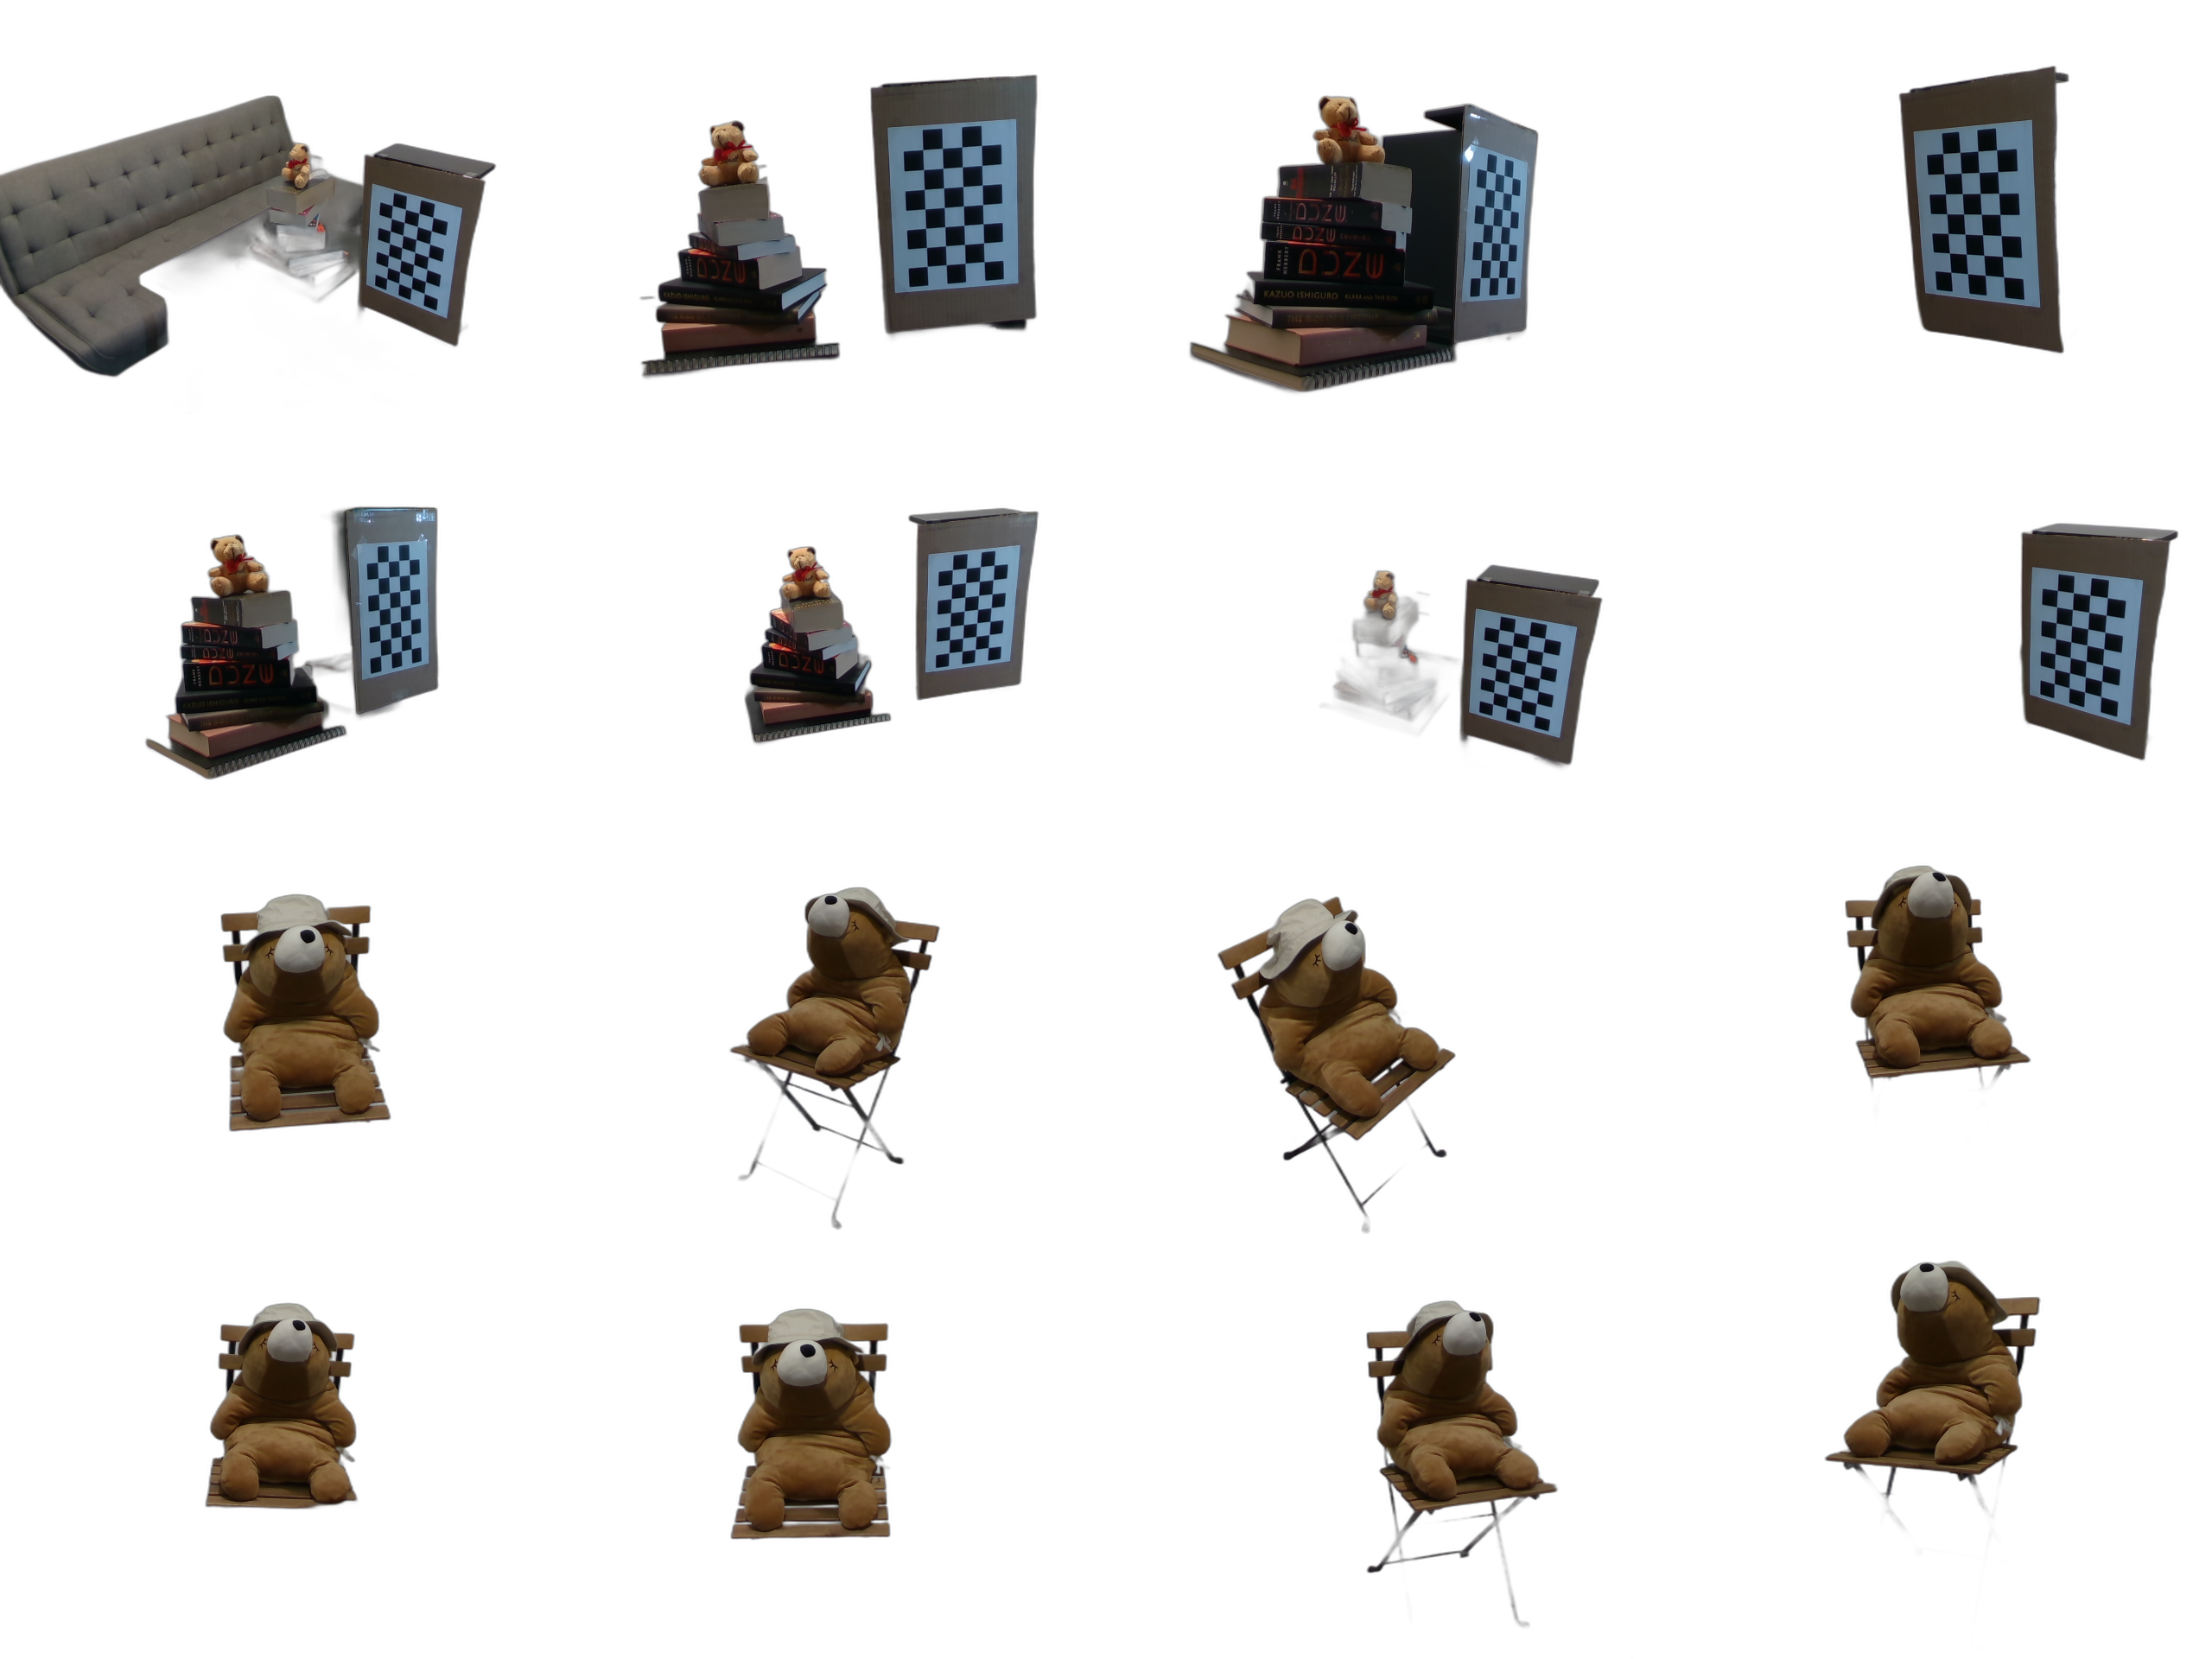
\includegraphics[width=\linewidth]{images/sample.png}
  \caption{Examples of background removal using U$^2$-Net.}
   \label{fig:sample}
\end{figure}


\section{Concluding Remarks}
In this project, we have assessed the empirical performance of using a stereoscopic depth sensor to estimate an initial point cloud for Point-NeRF in a variety of real-world settings. Our results suggest that the integration of coarse depth images into the Point-NeRF pipeline could serve as a promising and effective approach to enhance the quality of novel synthesized views. This approach maintains the advantages offered by Point-NeRF, such as faster convergence, improved scalability, and superior rendering quality compared to the vanilla NeRF method.

One important avenue for future work is the optimization of hyperparameters, and the comparison of the proposed and original methods on a wider variety of scenes. This will allow for a comprehensive evaluation of which settings are necessary for depth sensor initialization to outperform MVSNet initialization. Another direction to explore is the incorporation of depth images as supplementary inputs to MVSNet or other multiview stereo techniques, as this may enhance the accuracy of the pose estimations and point cloud reconstructions which Point-NeRF processes. Lastly, future work could also investigate the potential of using other inexpensive depth sensors, like structured light projection, to acquire depth images with higher precision and resolution.


% \begin{figure}[h]
%   \centering
%   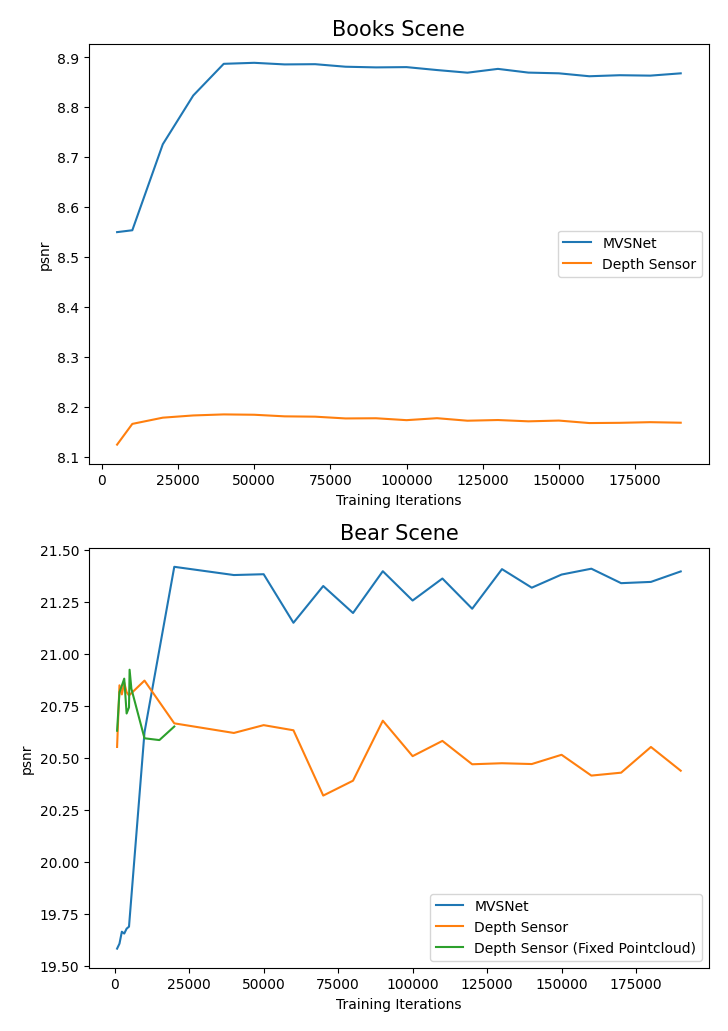
\includegraphics[width=\linewidth]{images/psnr.png}
%   \caption{PSNR during experiments.}
%    \label{fig:psnr}
% \end{figure}

% \begin{figure}[h]
%   \centering
%   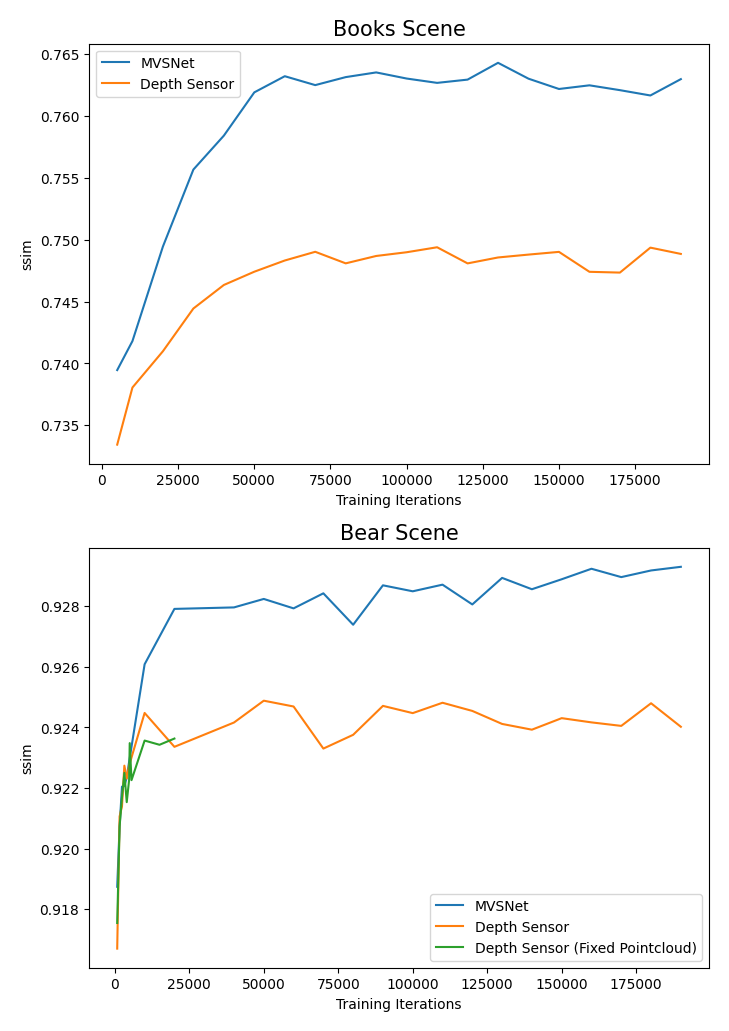
\includegraphics[width=\linewidth]{images/ssim.png}
%   \caption{SSIM during experiments.}
%    \label{fig:ssim}
% \end{figure}

% \begin{figure}[h]
%   \centering
%   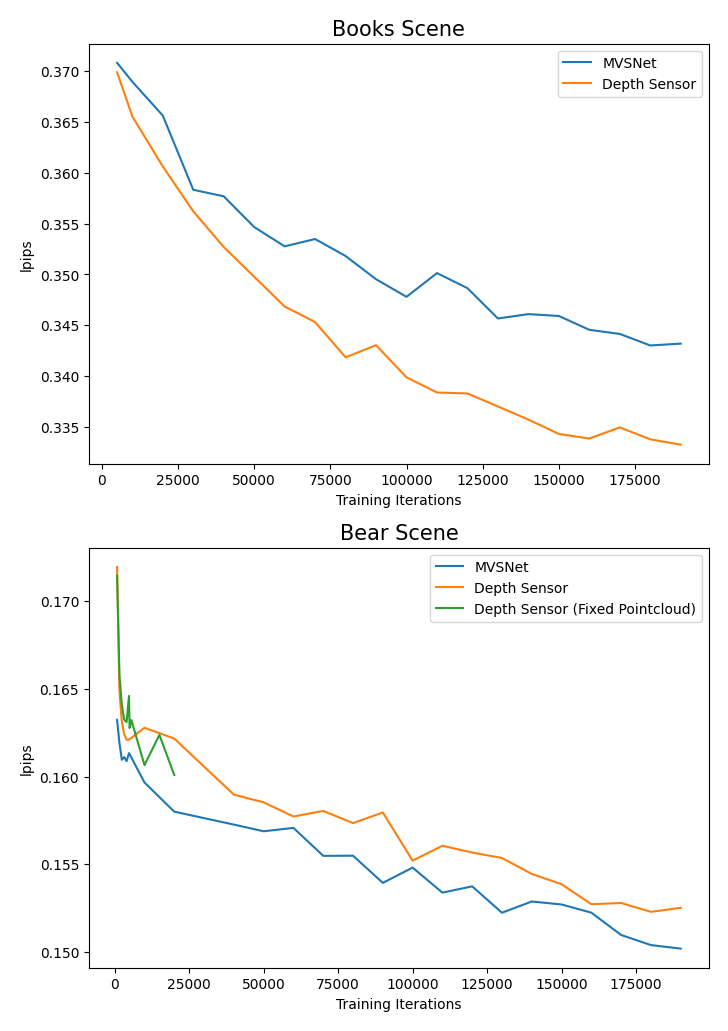
\includegraphics[width=\linewidth]{images/lpips.png}
%   \caption{LPIPS during experiments.}
%    \label{fig:lpips}
% \end{figure}


%%%%%%%%% REFERENCES
{\small
\bibliographystyle{ieee_fullname}
\bibliography{egbib}
}



\end{document}
